%!TEX root =  main.tex
\section{\dynastar: dynamic and quasi-optimum state partitioning}
%\section{\dynastar: dynamic partitioning for scalable state machine replication}
%\section{The centralized partitioning scheme}

%If the system can be modeled as a graph, as described in the previous session, we can take advantage of algorithms that perform graph partitioning to optimise the state partitioning of \ssmr\  while using concepts from \dssmr. The problem of graph partitioning is well stablished and despite being NP-Complete \ref{NPC_GraphPartition}, several approximation algorithms exist. First we define what graph partitioning is and how it can analyzed to our needs, next we explore possibilities that are easily obtainable when applying the same graph's reasoning.

\subsection{Overview}
%\subsection{State partitioning as a graph problem}

\dynastar extends the decentralized dynamic scheme proposed by Long et al.~\cite{hoang2016} to cope with workloads that exhibit both strong and weak locality.
In the presence of strong locality, \dynastar converges more quickly than the decentralized dynamic scheme.
Under weak locality (i.e., workloads that cannot be perfectly partitioned), \dynastar largely outperforms the decentralized dynamic scheme.
The key insights of \dynastar are to create the workload graph on-the-fly and use graph partitioning techniques to optimally relocate application state on-demand.
\begin{itemize}
\item \emph{On-the-fly workload modeling.}
\dynastar models a service workload as a graph $G = (V, E)$, where vertices represent state variables and edges commands.
An edge connecting two variables in the graph represents a command that accesses the variables. 
The oracle builds the workload graph based on feedback from the clients and partitions, as commands are executed.
\item \emph{On-demand application state relocation.}
Periodically, the oracle computes an ``ideal" partitioning of the workload graph.
Based on this partitioning and the current location of variables, the oracle computes the destination partition for commands that access variables spread on multiple partitions.
Variables are only moved on needed, the and the destination partition strives to minimize the number of moves. 
\end{itemize}




\subsection{The \dynastar protocol}

Algorithms~\ref{alg:client_proxy}, \ref{alg:server_proxy}, and \ref{alg:oracle_proxy} describe in detail how client, server and oracle processes execute, respectively.
For brevity, we omit the delete command since the coordination involved in the execution of a create and of a delete commands are analogous. 
Moreover, in the discussion in this section, every command involves the oracle.
In the next section, we explain how clients can use a caching technique to avoid using the oracle in the execution of most commands.

\begin{figure*}
\begin{minipage}[b]{1\linewidth} % A minipage that covers the whole width of the page
\centering
      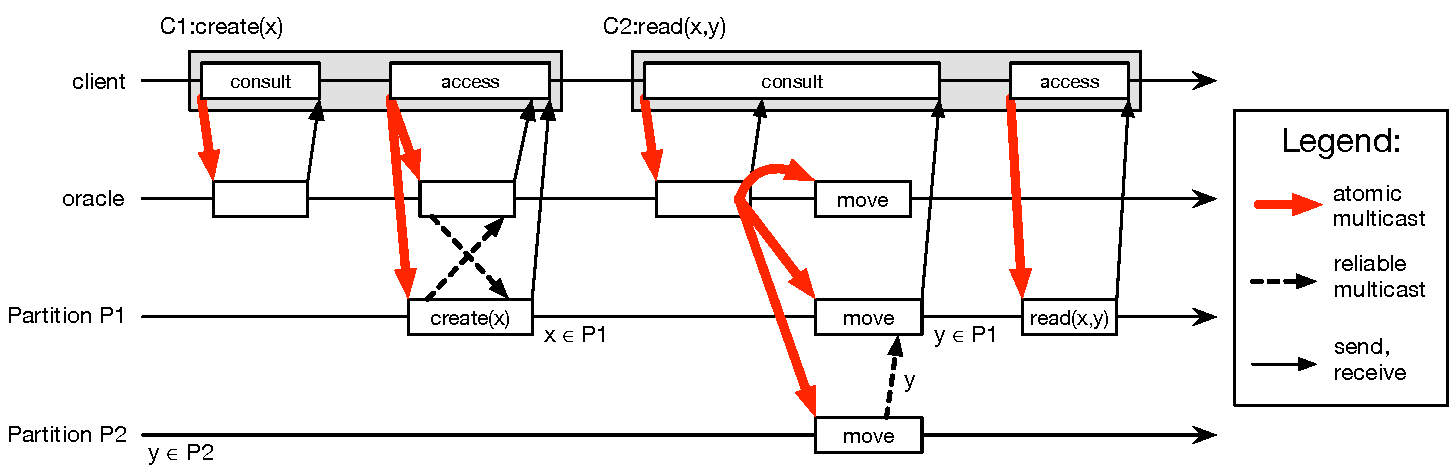
\includegraphics[width=0.9\linewidth]{figures/dynastar}
\end{minipage}
\caption{The execution of a create command and a read command in \dynastar.}
\label{fig:oracle_repartition}
\end{figure*}

%When issuing a command, the application simply forwards the command to the client proxy and waits for the reply.
%Consulting the oracle and multicasting the command to different partitions is done internally by the proxy at the client.
%Every server proxy at a server in $\ssm_i$ has only partial knowledge of the partitioning: it knows only which variables belong to $\ppm_i$.
%The oracle proxy has knowledge of every $\ppm \in \Psi$.
%To maintain such a global knowledge, the oracle must \amdel{} every command that creates, moves, or deletes variables.
%(In Section~\ref{sec:optm}, we introduce a caching mechanism to prevent the oracle from becoming a performance bottleneck.)

%\clearpage
\begin{algorithm}[h!]
\small

\begin{distribalgo}[1]

\vspace{1.0mm}

\INDENT{To issue a command $C$, the client proxy does:}

\vspace{1.0mm}

    \INDENT{\textbf{do}}
        \STATE \amcast$($oracle, $consult(C))$
        \STATE wait for $prophecy$
        \IF{$prophecy \in \{ok, nok\}$}
            \STATE $reply \leftarrow prophecy$
        \ELSE
            \STATE $C.vars \leftarrow \{v: \exists P : \langle v, P \rangle \in prophecy \}$
            \STATE $C.dests \leftarrow \{P: \exists v : \langle v, P \rangle \in prophecy \}$
            \IF{$C$ is an $access$ command and $|C.dests| > 1$}
                \STATE let $P_d$ be one of the partitions in $C.dests$
                \FOR{every $v \in C.vars$}
                    \STATE // \textit{move $v$ partition $P_d$}
                    \STATE let $P_o$ be $P : \langle v, P \rangle \in prophecy$
                    \IF{$P_o \neq P_d$}
                        \STATE $C_{move} \leftarrow move(v,P_d)$
                        \STATE $C_{move}.dests \leftarrow \{$oracle$,P_o,P_d\}$    
                        \STATE \amcast$(C_{move}.dests$, $C_{move})$
                    \ENDIF
                \ENDFOR
                \STATE $C.dests \leftarrow \{ P_s \}$
            \ENDIF
            \IF{$C$ is $create$ or $delete$}
                \STATE $C.dests \leftarrow dests \cup \{oracle\}$
            \ENDIF
            \STATE \amcast$(C.dests$, $C)$
            \STATE wait for $reply$
        \ENDIF
    \ENDINDENT
    \STATE{\textbf{while} $reply = retry$ // \textit{after $n$ retries, fall back to \ssmr}}
    \STATE return $reply$ to the application client
\ENDINDENT

\caption{\dssmr\ Client Proxy}
\label{alg:client_proxy}
\end{distribalgo}
\end{algorithm}
\begin{algorithm}[h!]
\small

\begin{distribalgo}[1]

\vspace{1.0mm}

\INDENT{To execute a command $C$, the server proxy in partition $\ppm$ does:}

    \vspace{1.0mm}
    
    \INDENT{\textbf{when} \rmdel$( \langle val, C \rangle )$}
        \STATE $rcvd\_msgs \leftarrow rcvd\_msgs \cup \{\langle val, C \rangle\}$
    \ENDINDENT

    \vspace{1.0mm}

    \INDENT{\textbf{when} \amdel$(C)$}

    \vspace{1.0mm}

        \IF{\underline{$C$ is an $access(\omega)$ command}}
            \IF{$\exists v \in \omega : v \not\in \ppm$}
                \STATE reply with $retry$
            \ELSE
                \STATE have the command executed by the application server
                \STATE send the reply to the client
            \ENDIF
        

        \vspace{1.0mm}
    
        \ELSIF{\underline{$C$ is a $move(v,\ppm_s,\ppm_d)$ command}}
            \IF{$\ppm = \ppm_s$}
                \IF{$v \in \ppm$}
                    \STATE \rmcast$(\ppm_d$,$\langle v, C \rangle)$
                    \STATE $\ppm \leftarrow \ppm \setminus \{v\}$
                \ELSE
                    \STATE \rmcast$(\ppm_d$,$\langle null, C \rangle)$
                \ENDIF
            \ELSE
                \STATE wait until $\exists val : \langle val, C \rangle \in rcvd\_msgs$
                \IF{$val \neq null$}
                    \STATE $v \leftarrow val$
                    \STATE $\ppm \leftarrow \ppm \cup \{v\}$
                \ENDIF
            \ENDIF
        
        \vspace{1.0mm}
    
        \ELSIF{\underline{$C$ is a $create(v)$ command}}
            \STATE wait until $\langle val, C \rangle \in rcvd\_msgs$
            \IF{$val = ok$}
                \STATE $\ppm \leftarrow \ppm \cup \{v\}$
%                \STATE reply with $success$
%            \ELSE
%                \STATE reply with $retry$
            \ENDIF
        
        \vspace{1.0mm}
        
        \ELSIF{\underline{$C$ is a $delete(v)$ command}}
            \IF{$v \in \ppm$}
                \STATE $\ppm \leftarrow \ppm \setminus \{v\}$
%                \STATE reply with $success$
%            \ELSE
%                \STATE reply with $retry$
            \ENDIF
        \ENDIF
    \ENDINDENT
\ENDINDENT

\caption{\dssmr\ Server Proxy}
\label{alg:server_proxy}
\end{distribalgo}
\end{algorithm}
\begin{algorithm}[t!]
\small

\begin{distribalgo}[1]

%\vspace{1.0mm}

	\INDENT[\textbf{Task 1}]{\colorbox{\coloralgo}{\textbf{when} \amdel$(consult(C))$}}
%		\INDENT{\textbf{case} $C$ is a $consult(C_c)$ command:}
%			\STATE $update(G_W, \omega)$
			\INDENT{\textbf{case} $C$ is a $create(v)$ command:}
				\IF[if $v$ already exists...]{$\parts(\{v\}) \neq \bot$}
					\STATE $prophecy \leftarrow nok$
					\COMMENT{...notify client}
				\ELSE[if $v$ doesn't exist...]
					\STATE $\ppm \leftarrow target(G_W, \{v\})$
					\COMMENT{...determine $v$'s partition}
					\STATE $prophecy \leftarrow (\{ \ppm, oracle \}, false)$
%					\COMMENT{prepare client's response}
				\ENDIF
			\ENDINDENT
			\INDENT{\textbf{case} $C$ is an $access(\omega)$ command:}
				\IF[if $v$ doesn't exist:]{$\exists v \in \omega : \parts(\{v\}) = \bot$}
					\STATE $prophecy \leftarrow nok$
					\COMMENT{tell the client}
				\ELSE[if all vars in $\omega$ exist]
%					\STATE $dests \leftarrow \emptyset$
%					\FOR{each $v \in \omega$}
%						\STATE $dests \leftarrow dests \cup partition(v)$
%					\ENDFOR
					\STATE $dests \leftarrow \parts(\omega)$
					\COMMENT{get all partition involved}
					\IF[if only one partition:]{$|dests| = 1$}
						\STATE $prophecy \leftarrow (dests,false)$
%						\COMMENT{tell client which partition}
					\ELSE[if multiple partitions involved]
						\STATE $\ppm_d \leftarrow target(G_W, \omega)$
						\COMMENT{$\ppm_d$ will store all vars in $\omega$}
						\STATE $alldest \leftarrow \{oracle\} \cup dests$
						\COMMENT{move $v$ from $\ppm_s$...}
						\STATE \amcast$(alldest, move(\omega,dests,\ppm_d))$
						\COMMENT{...to $\ppm_d$}						
%						\FOR[for each involved var $v$]{each $v \in \omega$}
%							\STATE $\ppm_s \leftarrow \parts(\{v\})$
%							\COMMENT{$\ppm_s$ is $v$'s current partition}
%							\IF[if $v$ not in $\ppm_d$:]{$\ppm_s \neq \ppm_d$}
%								\STATE $aux \leftarrow \{oracle,\ppm_s,\ppm_d\}$
%								\COMMENT{move $v$ from $\ppm_s$...}
%								\STATE \amcast$(aux$, $move(v,\ppm_s,\ppm_d))$
%								\COMMENT{...to $\ppm_d$}
%							\ENDIF 
%						\ENDFOR
						\STATE $prophecy \leftarrow (\{\ppm_d\},true)$
					\ENDIF 
				\ENDIF
			\ENDINDENT
			\STATE send $prophecy$ to the client
%			\INDENT{\textbf{case} $C_c$ is a $delete(v)$ command:}
%				\IF{$partition(v) = \bot$}
%					\STATE $prophecy \leftarrow ok$
%				\ELSE
%					\STATE $prophecy \leftarrow (\{ \ppm : v \in \ppm, oracle \}, -)$
%				\ENDIF
%			\ENDINDENT
%		\ENDINDENT
	\ENDINDENT
	\vspace{1.0mm}

	\INDENT[\textbf{Task 2}]{\colorbox{\coloralgo}{\textbf{when} \amdel$(create(v))$}}
%	\INDENT{\textbf{case} $C$ is a $create(v)$ command:}
		\STATE let $\ppm_c \in C.dests \setminus \{oracle\}$
		\COMMENT{var created in $\ppm_c$}
		\STATE \rmcast$(\ppm_c, \langle signal, C \rangle )$
		\COMMENT{exchange signal to...}
		\STATE wait until $\langle signal, C \rangle \in rcvd\_msgs$
		\COMMENT{...coordinate partitions}
		\STATE $\ppm_c \leftarrow \ppm_c \cup      \{v\}$
                \STATE send $ok$ to the client
	\ENDINDENT

	\vspace{1.0mm}
	\INDENT[\textbf{Task 3}]{\colorbox{\coloralgo}{\textbf{when} \amdel$(move(\omega,dests,\ppm_d))$}}
%        \INDENT{\textbf{case} $C$ is a $move(v,\ppm_s,\ppm_d)$ command:}
                \STATE \textbf{for} each $\ppm_s \in dests$ \textbf{do} $\ppm_s \leftarrow \ppm_s \setminus \omega$
                \COMMENT{update partitions...}
                \STATE $\ppm_d \leftarrow \ppm_d \cup \omega$
                \COMMENT{...and add new variables}
                \STATE send $ok$ to the client
	\ENDINDENT

        \vspace{1.0mm}
    
	\INDENT[\textbf{Task 4}]{\colorbox{\coloralgo}{\textbf{when} \rmdel$( \langle val, C \rangle )$}}
		\STATE $rcvd\_msgs \leftarrow rcvd\_msgs \cup \{\langle val, C \rangle\}$
	\ENDINDENT
	
	\vspace{1.0mm}
	\INDENT{\colorbox{\coloralgo}{\textbf{function} \parts$(vars)$}}
		\STATE $aux \leftarrow \{ \ppm : \exists v \in vars \cap \ppm \}$
		\STATE return $aux$
	\ENDINDENT
	
%	\vspace{1.0mm}
	\rule{83mm}{0.4pt}
%	\vspace{0.1mm}

	\INDENT[\textbf{Task 5}]{\colorbox{\coloralgo}{\textbf{when} \amdel$(hint(V_h,E_h))$}}
		\STATE update $G_W$ with $(V_h,E_h)$
%		\STATE send $ok$ to the client
	\ENDINDENT
	
	\vspace{1.0mm}
    
	\INDENT[\textbf{Task 6}]{\colorbox{\coloralgo}{\textbf{periodically} do}}
		\STATE compute ideal partition $\ip_1, ..., \ip_m$ from $G_W$
	\ENDINDENT
	
	\vspace{1.0mm}
    
	\INDENT{\colorbox{\coloralgo}{\textbf{function} target$(vars)$}}
		\STATE $\ppm \leftarrow$ compute destination partition for $vars$ from\\ \hspace{8mm}current $\ppm_1, ..., \ppm_m$ and ideal $\ip_1, ..., \ip_m$ partitionings
		\STATE return $\ppm$
	\ENDINDENT	
	
%	\vspace{1.0mm}
%        
%	\INDENT{\textbf{case} $C$ is a $delete(v)$ command:}
%		\STATE let $\ppm_d$ be $\ppm : \{\ppm\} = C.dests \setminus \{$oracle$\}$
%		\STATE $\ppm_c \leftarrow \ppm_c \setminus      \{v\}$
%		\STATE \rmcast$(\ppm_c, \langle ok, C \rangle )$
%			\STATE wait until $\exists val : \langle val, C \rangle \in rcvd\_msgs$
%	\ENDINDENT

%\ENDINDENT

\caption{Oracle}
\label{alg:oracle_proxy}
\end{distribalgo}
\end{algorithm}



\subsubsection{The client process} 

To execute a command, the client atomically multicasts the command to the oracle in a consult message to find out the partitions involved.
The oracle replies with a prophecy, which may already tell the client that the command cannot be executed (e.g., it needs a variable that does not exist, it tries to create a variable that already exists).
If the command can be executed, the client receives a prophecy containing a tuple $(dests, sync)$, where $dests$ is a set of the partitions the command must be atomically multicast to for execution, and $sync$ is a flag that tells the client whether it must coordinate with a partition before atomically multicasting the command.
This happens if the oracle requests variables to be moved to a single destination partition, in which case the client must wait for the destination partition to receive the variables.

After the client atomically multicasts the command to the destination partition, it waits for a response from the servers in the partition.
The client must retry the command if the partition cannot execute the command.
This happens if some of the variables needed by the command were moved to another partition due to other commands. 
To ensure that a command is eventually executed, after retrying a few times, the client falls back \ssmr{}, multicasting the command to all partitions (and the oracle, in case of a create or delete command).

\subsubsection{The server process} 

When a server delivers a command for execution, it first checks that all variables accessed by the command are stored locally, in which case the command is executed and the response is sent back to the client (Task 1 in Algorithm~\ref{alg:server_proxy}).
If one or more variables are not stored at the partition, the server returns a message to the client to retry the operation.
This happens if some variables have been moved to another partition due to another command. 

Upon delivering a message to move variables (Task 2), a server in the source partition reliably multicasts all the needed variables stored locally to the destination partition (possibly none, if these variables have already been moved).
Servers in the destination partition simply wait for a message from each source partition.

When a server delivers a message to create a variable (and similarly to delete an existing variable), it coordinates with the oracle (Task 3).
The exchange of signals between the partition where the variable will be created and the oracle ensures that interleaved executions between create and delete commands will not lead to violations of linearizability (i.e., this is essentially the execution of a multi-partition command involving the oracle and a partition~\cite{bezerra2014ssmr}).

\subsubsection{The oracle} 

When the oracle delivers a consult request (Task 1 in Algorithm~\ref{alg:oracle_proxy}), it distinguishes between two cases.
\begin{itemize}
\item If the command is to create a variable $v$, the oracle checks that the $v$ does not already exist, in which case the oracle determines the destination partition of $v$ and returns a response to the client.
In the case of a create, the oracle chooses a random partition for the new variable.
\item If the command is not a create, the oracle first checks that all variables involved in the command exist.
If the variables exist and they are all in a single partition, the oracle returns to the client a prophecy with the partition the command must be atomically multicast to for execution.
If the variables accessed by the command are distributed in multiple partitions, the oracle determines the destination partition and atomically multicasts a move command to all such partitions and to the destination partition.
\end{itemize}

The oracle executes a create command (Task 2) by updating its partition information and coordinating with the destination partition of the variable.
This is done to avoid interleaved executions with other commands, which could lead to consistency violations. 
To execute a move command (Task 3), the oracle simply updates its local information about source and destination partitions.
In the case of a move command, the oracle does not coordinate with the involved partitions.
This is not necessary because a move cannot interleave its execution with a create and interleaved executions with other move commands simply result in retries by the clients.

The oracle also keeps track of the workload graph, periodically computes the ``ideal" partitioning of the graph, and determines the destination partition for move operations.
To maintain the workload graph (Task 5), the oracle receives hints with variables (i.e., vertices in the graph) and executed commands (i.e., edges in the graph).
These hints can be submitted by the clients (e.g., after the execution of a command), or by the partitions, which collect data upon executing commands and periodically inform the oracle.
In our social network application, clients inform the oracle upon submitting ``structural operations" on the social graph, that is, operations that change the  graph (i.e., follow and unfollow requests).

To ensure that the ideal partitioning periodically computed by the oracle replicas is deterministic (Task 6), each replica triggers the partitioning upon delivering a constant number of hints.
Moreover, the algorithm used to compute the partitioning of the graph must be also deterministic.
To determine the destination partition of a set of variables, as part of a move, the oracle chooses the partition that results in the minimum number of variables that need to be moved given the ideal partitioning and the current location of the variables.

\subsection{Performance optimizations}
\label{sec:optm}

In the algorithm presented in the previous section, clients always need to consult the oracle to determine the partition a command must be atomically multicast to for execution.
Obviously, if every command involves the oracle, the system is unlikely to scale, as the oracle will likely become a bottleneck.
To address this issue, clients are equipped with a location cache.
Before submitting a consult request to the oracle, the client checks its location cache.
If the cache contains the partition of the variables needed by the command and all variables are in a single destination partition, the client can atomically multicast the command to the partition and avoid contacting the oracle. 

The client needs to contact the oracle if not all variables needed by the command are in the same partition, or if the cache contains outdated information, or the command is a create, in which case it must involve the oracle, as explained before.
If the cache contains outdated information and the addressed partition does not contain all the variables accessed by the command, the partition tells the client to retry the command.
In this case, the client contacts the oracle and then updates its cache with the oracle's response.


\subsection{Correctness}
\label{sec:correctness}

In this section, we argue that \dssmr\ ensures termination and linearizability.
By ensuring termination, we mean that for every command $C$ issued by a correct client, a reply to $C$ different than $retry$ is eventually received by the client.
This assumes that at least one oracle process is correct and that every partition has at least one correct server.
Given these constraints, the only thing that could prevent a command from terminating would be an execution that forced the client proxy to keep retrying a command.
This problem is trivially solved by falling back to \ssmr\ after a predefined number of retries: at a certain point, the client proxy multicast the command to all server and oracle processes, which execute the command as in \ssmr{}, i.e., with coordination among all partitions and the oracle.

As for linearizability, we argue that, if every command in execution \ex\ of \dssmr\ is delivered by atomic multicast and is \emph{execution atomic} (as defined in~\cite{bezerra2014ssmr}), then \ex\ is linearizable.
We denote the order given by atomic multicast by relation $\prec$.
Given any two messages $m_1$ and $m_2$, ``$m_1 \prec m_2$'' means that there exists a process that delivers both messages and $m_1$ is delivered before $m_2$, or there is some message $m'$ such that $m_1 \prec m'$ and $m' \prec m_2$, which can be written as \mbox{$m_1 \prec m' \prec m_2$}.
%\fxnote[draft]{use the phrase \"there exists a process that\" }
Also, for the purposes of this proof, we consider the oracle to be a partition, as it also \amdel{}s and executes application commands.

Suppose, by means of contradiction, that there exist two commands $x$ and $y$, where $x$ finishes before $y$ starts, but $y \prec x$ in the execution.
There are two possibilities to be considered: (i) $x$ and $y$ are delivered by the same process $p$, or (ii) no process delivers both $x$ and $y$.

In case (i), at least one process $p$ delivers both $x$ and $y$.
As $x$ finishes before $y$ starts, then $p$ delivers $x$, then $y$. From the properties of atomic multicast, and since each partition is mapped to a multicast group, no process delivers $y$, then $x$.
Therefore, we reach a contradiction in this case.

In case (ii), if there were no other commands in \ex, then the execution of $x$ and $y$ could be done in any order, which would contradict the supposition that $y \prec x$.
Therefore, there are commands $z_1, ..., z_n$ with atomic order $y \prec z_1 \prec \cdots \prec z_n \prec x$, where some process $p_0$ (of partition $\ppm_0$) delivers $y$, then $z_1$; some process $p_1 \in \ppm_1$ delivers $z_1$, then $z_2$, and so on: process $p_i \in \ppm_i$ delivers $z_{i}$, then $z_{i+1}$, where $1 \leq i < n$.
Finally, process $p_n \in \ppm_n$ delivers $z_n$, then $x$.

Let $z_0 = y$ and let $atomic(i)$ be the following predicate:
``For every process $p_i \in \ppm_i$, $p_i$ finishes executing $z_i$ only after some $p_0 \in \ppm_0$ started executing $z_0$.''
We now claim that $atomic(i)$ is true for every $i$, where $0 \leq i \leq n$.
We prove our claim by induction.





